\documentclass[12pt,letterpaper,titlepage]{article}

\usepackage{fontspec}
\defaultfontfeatures{Mapping=tex-text}
\usepackage{xunicode}
\usepackage{xltxtra}
\usepackage{amsmath}
\usepackage{pdfpages}
\usepackage{amsfonts}
\usepackage{bbold}
\usepackage{amssymb}
\setcounter{secnumdepth}{0}
\usepackage{nameref}
\usepackage{enumitem}
\usepackage{environ}
\usepackage{pgfplots}
\usepackage{listings}

\showboxdepth=\maxdimen
\showboxbreadth=\maxdimen


\usepackage{paracol}
\usepackage{wrapfig}
\globalcounter{table}
\globalcounter{figure}
\usepackage{graphicx}
\usepackage[left=1in,right=1in,top=1in,bottom=1in]{geometry}
\graphicspath{{img/}}

\author{Jacob Abel}
\title{	Homework 3
	\\\large ECE2500 CRN:82943
}

\setlength{\parskip}{0.5em}

\begin{document}
\maketitle
\begin{raggedright}

\paragraph{Problem 1: }
Arrange the following branch/jump instructions in descending order of their maximum possible jump target. That is, the instruction that allows the farthest possible jump must go first, followed by the next farthest, and so on. If two instructions allow the same amount of jump, list them in any order. Also state encoding format (R/I/J) and the number of bits used to represent the target address for each instruction. Finally, list for each instruction the maximum distance that can be jumped, both forwards and backwards in memory.

\begin{lstlisting}
j, beq, jr, jal, bne
\end{lstlisting}

\begin{enumerate}
\item[jr]
\begin{description}
\item[Encoding Format: ] Register
\item[Address Bits: ] 32-bit
\item[Max Direct Jump Address: ] \texttt{0xFFFFFFFF}
\item[Range] Any location within 32-bit addressable memory.
\end{description}
\item[jal]
\begin{description}
\item[Encoding Format: ] Jump
\item[Address Bits: ]
\item[Max Direct Jump Address: ] \texttt{0xFFFFFFF}
\item[Range] Any location with the same upper 4 bits.
\end{description}
\item[j]
\begin{description}
\item[Encoding Format: ] Jump
\item[Address Bits: ] 26-bit
\item[Max Direct Jump Address: ] \texttt{0xFFFFFFF}
\item[Range] Any location with the same upper 4 bits.
\end{description}
\item[beq]
\begin{description}
\item[Encoding Format: ] Immediate
\item[Address Bits: ] 16-bit
\item[Max Forward Distance: ] \texttt{0x7FFF}
\item[Max Backward Distance: ] \texttt{0x8000}
\end{description}
\item[bne]
\begin{description}
\item[Encoding Format: ] Immediate
\item[Address Bits: ] 16-bit
\item[Max Forward Distance: ] \texttt{0x7FFF}
\item[Max Backward Distance: ] \texttt{0x8000}
\end{description}
\end{enumerate}

\clearpage

\paragraph{Problem 2: }
Answer true or false to the following questions and give reasons: 
\begin{enumerate}
\item The immediate constant operand in the sltiu instruction is treated as an unsigned 16-bit integer. 

Yes as it is an unsigned instruction.

\item The immediate constant operand in the sltiu instruction is sign extended. 

Yes as all arithmetic immediate instructions are sign extended whether or not they are signed.

\end{enumerate}

\paragraph{Problem 3: } 
Suppose the program counter (PC) is set to \texttt{0x30002000}. Is it possible to use the jump (j) MIPS assembly instruction to jump directly to the instruction at \texttt{0x50003000}? If yes, write the corresponding assembly instruction(s). If not, explain why and give other MIPS instruction(s) that can jump to this target address. (For this problem, assume that the instruction memory starts from \texttt{0x00000000} and goes to \texttt{0xFFFFFFFF}.)

No as jump can only access the same $256\text{ MB}_2$ of memory block as the program counter and the intended location is in a different block. Jump register has full 32-bit memory access and can reach said address. The following would get to the address.

\begin{lstlisting}
lui  $t0 0x5000
ori  $t0 0x3000
jr   $t0
\end{lstlisting}

\paragraph{Problem 4: }
 The mul3.asm file gives the assembly code that implements the main function which calls the mul3 function by passing three arguments in $\$a0$, $\$a1$, $\$a2$. mul3 returns the solution (product of the three input arguments) in $\$v0$ (which is then saved in $\$s0$). Modify this function so that instead of taking in three arguments, the function takes in six input arguments. The output should be the product of all six input arguments. You must use the stack (i.e., use the memory with the $\$fp$ register and/or $\$sp$ register) to pass the input arguments. Your submission must consist of a file named mul6.asm with the modified code. Test your code in QtSPIM. In both the screenshots, mark the data that your code pushed onto the stack. In addition, in the pdf report state the following values from QtSPIM: $\$ra$ register before and after executing the jal instruction and $\$fp$ and $\$sp$ registers before pushing any argument on the stack, after pushing all six arguments on the stack (but before jal), and after popping all six arguments from the stack in mul6.

\paragraph{$\$fp$} Unused for this problem.
\begin{paracol}{2}
\paragraph{$\$sp$}
\begin{description}[noitemsep]
\item[Before:] \texttt{0x7FFFEED0}
\item[After: ] \texttt{0x7FFFEEC0}
\end{description}
\switchcolumn
\paragraph{$\$ra$}
\begin{description}[noitemsep]
\item[Before:] \texttt{0x400018}
\item[After: ] \texttt{0x40005c}
\end{description}
\end{paracol}
\clearpage

\begin{enumerate}
\item User stack at the start of the program (before pushing anything on the stack).
\begin{center}
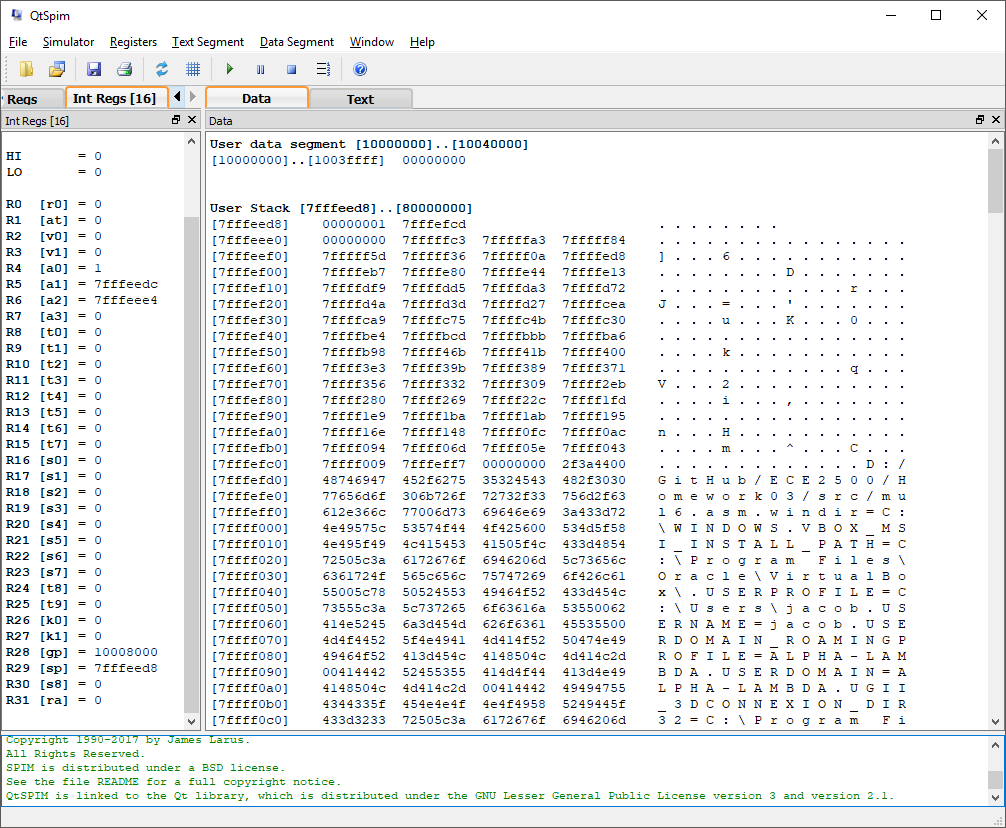
\includegraphics[width=\textwidth, height=20\baselineskip, keepaspectratio=true]{pre}
\end{center}

\item User stack after pushing all six arguments on the stack.
\begin{center}
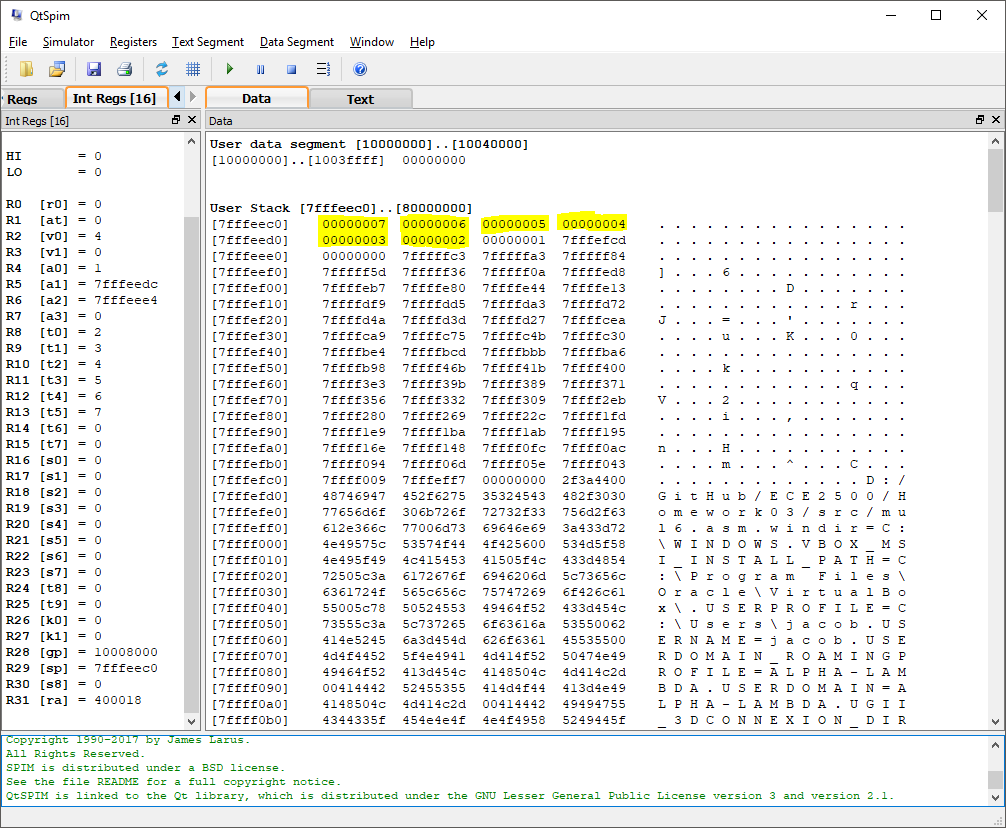
\includegraphics[width=\textwidth, height=20\baselineskip, keepaspectratio=true]{post}
\end{center}

\end{enumerate}

\end{raggedright}
\end{document}